\documentclass[a4paper,11pt,titlepage]{article}
% The maths package
\usepackage{amsmath}
\usepackage{amsfonts}
% The graphics package
\usepackage{graphicx}
% Allows paragraph in blocks
\usepackage{parskip}
% Code hightling
\usepackage{minted}
% Verbatim file inclusion
\usepackage{fancyvrb}

%%%% Define the title %%%%%%%%%%%%%%%%%%%%%%%%%%%%%%%%%%%%%%%%%%%%%%%%%%%%%%%%%%
\title{
MECH3750 Engineering Analysis II \\ 
Assignment 2
}
% define the author
\author{
Merrick Heley\\
42339915
}

%%%% Notes, commands, settings %%%%%%%%%%%%%%%%%%%%%%%%%%%%%%%%%%%%%%%%%%%%%%%%%
% \section*{Task 1} uses an asterisk to suppress the section number

% This command adds \ud for finishing integrals
\newcommand{\ud}{\,\mathrm{d}}

% Set the pygmentation style for code
% pygmentize -L styles
\usemintedstyle{autumn}

% Simple command for python file input
\newcommand{\inputpython}[1]{
    \inputminted[linenos=true, 
                 frame=single, 
                 fontsize=\scriptsize, 
                 label=#1]
                {python}{#1}
}

% Simple command for python file output
\newcommand{\pythonoutput}[1]{
    \immediate\write18{python #1 > #1.out}
    \fvset{frame=single, numbers=left, fontsize=\scriptsize, label=#1.out}
    \VerbatimInput{#1.out}
    \write18{del #1.out}
}

% Simple command for python file input
\newcommand{\inputmaxima}[1]{
    \inputminted[linenos=true, 
                 frame=single, 
                 fontsize=\scriptsize, 
                 label=#1]
                {cpp}{#1}
}

%%%% Start document %%%%%%%%%%%%%%%%%%%%%%%%%%%%%%%%%%%%%%%%%%%%%%%%%%%%%%%%%%%%

\begin{document}
% generates the title
\maketitle

%%%% Question 0.1 %%%%%%%%%%%%%%%%%%%%%%%%%%%%%%%%%%%%%%%%%%%%%%%%%%%%%%%%%%%%%%
\section*{Question 0.1: Boundary Value Problems}
\subsection*{a. Shooting Method}

\subsection*{b. Lehmer-Shur Algorithm}

\subsection*{c. Difference Method}

\begin{align}
-y'''(x) + y''(x) - 4xy'(x) + (8x + 3)y(x) &= x^2 \label{eq:q1bvp}\\
y(-1) & = -10 \notag\\
y(0.5) & = 1 \notag\\
y(1.5) & = -3 \notag
\end{align}

To solve this boundary value problem using difference method, approximations 
must be formed using a difference approximation. To keep the problem simple, a 
first order central difference method was initially used.

\begin{align}
y' & = \frac{1}{2h}(y_{i+1} - y_{i-1}) \label{eq:central1}\\
\intertext{When this equation is substituted into itself, it can be derived 
            further}
y'' & = \frac{1}{h^2}(y_{i+1} - 2y_i + y_{i-1}) \label{eq:central2}\\
\intertext{And once more}
y''' & = \frac{1}{2h^3}(y_{i+2} - 2y_{i+1} + 2y_{i-1} - y_{i-2}) 
            \label{eq:central3}
\end{align}

Substituting \eqref{eq:central1} \eqref{eq:central2} 
            \eqref{eq:central3} into \eqref{eq:q1bvp} \\
\begin{equation*}
-\frac{1}{2h^3}(y_{i+2} - 2y_{i+1} + 2y_{i-1} - y_{i-2}) 
+ \frac{1}{h^2}(y_{i+1} - 2y_i + y_{i-1})
- \frac{4x}{2h}(y_{i+1} - y_{i-1})
+ (8x + 3)y_i
= x_i^2
\end{equation*}

And rearranging to group $y_i$ values together

\begin{equation}
\left(\frac{1}{2h^3}\right)y_{i-2} + 
\left(\frac{-2}{2h^3} + \frac{1}{h^2} + \frac{4x}{2h}\right)y_{i-1} +
\left(\frac{-2}{h^2} + (8x + 3)\right)y_i +
\left(\frac{2}{2h^3} + \frac{1}{h^2} + \frac{-4x}{2h}\right)y_{i+1} +
\left(\frac{-1}{2h^3}\right)y_{i-2}
= x_i^2
\end{equation}


\inputpython{Task1c.py}
\pythonoutput{Task1c.py}

\begin{figure}[!hbp]
\centering
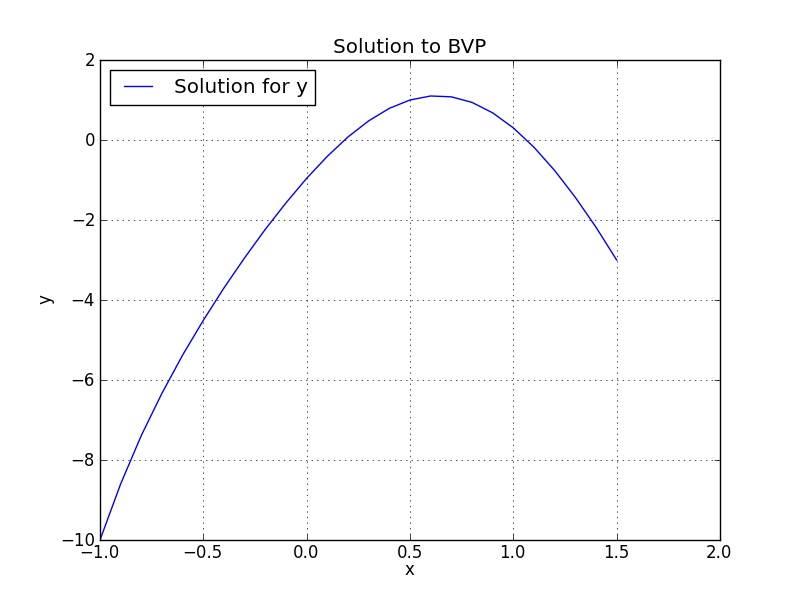
\includegraphics[scale=0.5]{Task1c.png}
\caption{Solution to BVP using Difference Method}
\end{figure}

\subsection*{d. Non-Linear Difference Method}

%%%% Question 0.2 %%%%%%%%%%%%%%%%%%%%%%%%%%%%%%%%%%%%%%%%%%%%%%%%%%%%%%%%%%%%%%
\section*{Question 0.2: Newtons Method}
\subsection*{a. Single Solution}

\subsection*{b. Solutions in $\mathbb{C}$}

\subsection*{c. Proof of number of solutions}

\subsection*{d. Maxima Brute-force}
\inputmaxima{Task2d.wxm}

%%%% APPENDICES %%%%%%%%%%%%%%%%%%%%%%%%%%%%%%%%%%%%%%%%%%%%%%%%%%%%%%%%%%%%%%%%
\clearpage
\section*{Appendix A}
% Bisection method in appendix (shitty, and not correct way of doing appendices)
\inputpython{secant.py}
\pythonoutput{secant.py}



\clearpage
\end{document}